\section{Auswertung}
\label{sec:Auswertung}

Die in den Messungen verwendeten Zylinder und Platten werden mithilfe einer Schieblehre vermessen und haben die folgenden Dicken $d$.
Dabei werden die Werte als fehlerfrei angenommen.
\begin{description}
  \item[Zylinder 1] \SI{3.10}{\centi\meter}
  \item[Zylinder 2] \SI{3.97}{\centi\meter}
  \item[Zylinder 3] \SI{8.03}{\centi\meter}
  \item[Zylinder 4] \SI{10.20}{\centi\meter}
  \item[Zylinder 5] \SI{12.05}{\centi\meter}
  \item[Platte 1] \SI{0.61}{\centi\meter}
  \item[Platte 2] \SI{1.00}{\centi\meter}
\end{description}

\subsection{Bestimmung der Schallgeschwindigkeit und der Dämpfungskonstante mit dem Impuls-Echo-Verfahren}
\label{sub:ImpEch}
Zur Bestimmung der Schallgeschwindigkeit wird Platte 1 benutzt und dann die Laufzeit $t$ gemessen und in \autoref{tab:ImpLaufzeit} eingetragen.
Die Schallgeschwindigkeit $c$ wird mit \autoref{eqn:Strecke} berechnet, indem die Formel nach $c$ umgestellt und der dadurch berechnete Wert auch in \autoref{tab:ImpLaufzeit} 
eingetragen wird.

\begin{table}[H]
  \centering
  \caption{Laufzeit und Schallgeschwindigkeit durch Platte 1.}
  \label{tab:ImpLaufzeit}
  \sisetup{table-format=2.2}
  \begin{tabular}{S[table-format=1.0] S[table-format=1.0] S[table-format=2.0] S[table-format=4.0] }
  \toprule
  {Messung} & {Laufzeit $\Delta t / \si{\micro\second}$} & {Zeit $\Delta t / \si{\micro\second}$} & {Schallgeschwindigkeit $c / \frac{\si{meter}}{\si{\second}}$}\\
  \midrule
  1: &  5   & 5 & 2440  \\
  2: &  10  & 5 & 2440  \\
  3: &  14  & 4 & 3050  \\
  4: &  19  & 5 & 2440  \\
  \bottomrule
  \end{tabular}
\end{table}
Der Mittelwert der Schallgeschwindigkeit wird mit 
\begin{equation}
  \bar{c}=\frac{1}{n} \sum_{i=1}^n c_i \label{eqn:Mittelwert}
\end{equation}
zu
\begin{align*}
  \bar{c}=2592,5 \si{\meter\per\second}.
\end{align*}
Die Abweichung lässt sich mit
\begin{equation}
  \Delta \bar{c} = \frac{\sqrt{\frac{1}{n-1}\sum_{j=1}^n (c_j-\bar{c})^2}}{\sqrt{n}} \label{eqn:standabw}
\end{equation}
berechnen, sodass sich die mittlere Schallgeschwindigkeit zu
\begin{align*}
  \bar{c}= (2592,5 \pm 305) \si{\meter\per\second}
\end{align*}
ergibt.

\begin{figure}[H]
  \centering
  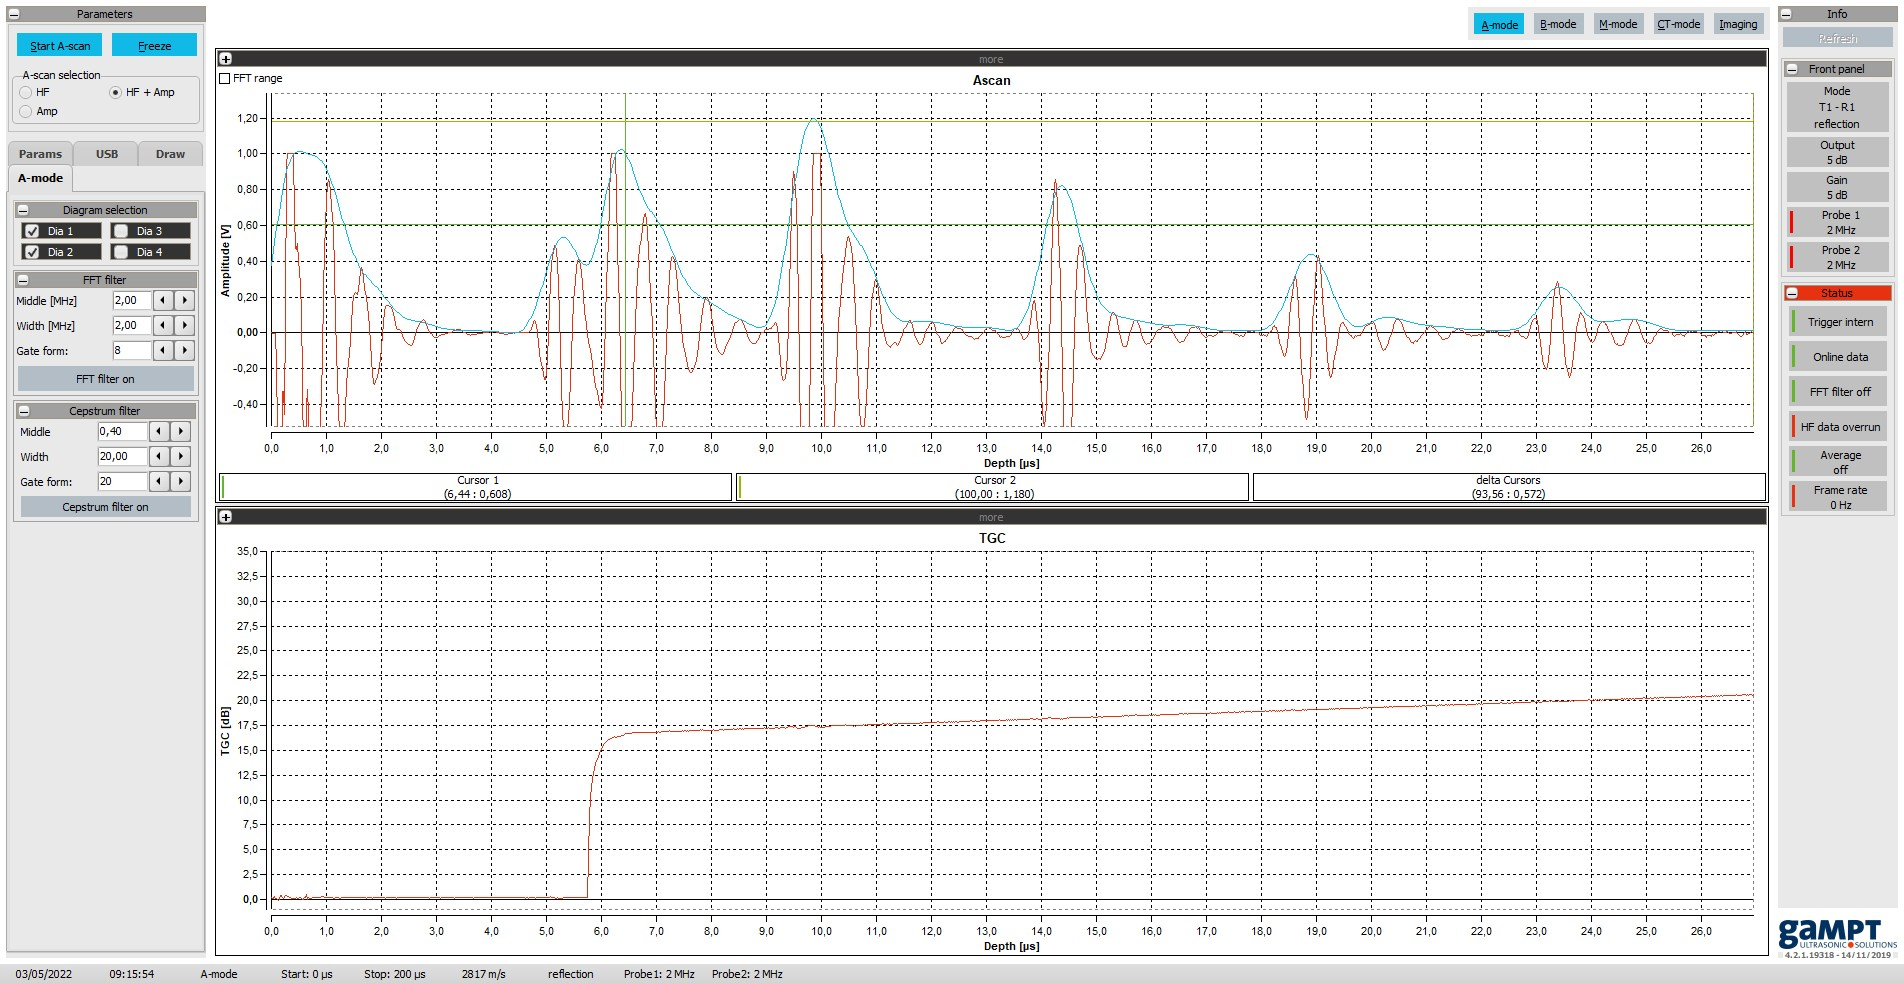
\includegraphics{build/Scan1.jpg}
  \caption {Abbildung des A-Scans der Acrylplatte 1.}
  \label{fig:scan1}
\end{figure}
Anhand von \autoref{fig:scan1} kann zwischen $5$ Schwingungen die Periode abgelesen werden und die Frequenz daraus bestimmt werden.
Die gemessene Periode $T$ wird mit der daraus nach
\begin{align*}
  f&= \frac{1}{T}
\end{align*}
berechneten Frequenz $f$ und der nach
\begin{align*}
  \lambda &= \frac{c}{f}
\end{align*} 
berechneten Wellenlänge $\lambda$ sind in \autoref{tab:Tfc} eingetragen.
Die Abweichung der Wellenlänge wird mit der Gaußschen Fehlerfortpflanzung
\begin{equation*}
  \Delta \lambda =\sqrt{\sum_{j=1}^n \left(\frac{1}{f} \cdot \Delta \bar{c} \right)^{2} }\label{eqn:Gauß}
\end{equation*}
bestimmt.
\begin{table}[H]
  \centering
  \caption{Periode, Frequenz und Wellenlänge.}
  \label{tab:Tfc}
  \sisetup{table-format=2.2}
  \begin{tabular}{S[table-format=1.1] S[table-format=1.1] S[table-format=4.2] @{${}\pm{}$} S[table-format=3.2] }
  \toprule
   {Periode $T / \si{\micro\second}$} & {Frequenz $f/ \si{\mega\Hz}$} & \multicolumn{2}{c}{Wellenlänge $\lambda /\si{\meter}$}\\
  \midrule
    0.4  & 2.5 & 1037.00 & 122.41 \\ 
    0.6  & 1.7 & 1525.00 & 179.41 \\
    0.6  & 1.7 & 1525.00 & 179.41 \\
    0.5  & 2.0 & 1296.25 & 152.50 \\
  \bottomrule
  \end{tabular}
\end{table}

Die Mittelwerte der Frequenz und der Wellenlänge betragen somit analog zu \autoref{eqn:Mittelwert} und \autoref{eqn:standabw} 
\begin{align*}
  \bar{f} &= 
  \bar{\lambda} &= 
\end{align*}

Der erste berechnete Wert der Schallgeschwindigkeit in Acryl $c=2440 \frac{\si{meter}}{\si{\second}}$ wird in das Darstellungsprogramm eingegeben.
Es wird eine Tiefenmessung durchgeführt. Die ersten beiden Peaks lagen bei $0.6 \si{\centi\meter}$ und $1.2 \si{\centi\meter}$, woraus abzulesen ist, dass die 
verwendete Platte eine Dicke von $d=0.6\si{\centi\meter}$ hat.\\

In der zweiten Messreihe werden die zuvor ausgemessenen Acrylzylinder mithilfe des Impuls-Echo-Verfahrens gemäß \autoref{sec:Durchführung} vermessen.
Die Ergebnisse der Messung sind in \autoref{tab:tAimpE} aufgelistet.
\begin{table}[H]
  \centering
  \caption{Laufzeit und Amplituden durch verschiedene Zylinder mit dem Impuls-Echo-Verfahren.}
  \label{tab:tAimpE}
  \sisetup{table-format=2.2}
  \begin{tabular}{S[table-format=1.0] S[table-format=2.0] S[table-format=1.2] }
  \toprule
  {Zylinder} & {Laufzeit $t / \si{\micro\second}$} &  {Amplitude $A / \si{\volt}$}\\
  1 &  24  & 1.24  \\
  2 &  30  & 1.24  \\
  3 &  59  & 0.24  \\
  4 &  76  & 0.08  \\
  \bottomrule
  \end{tabular}
\end{table}
Die Werte der Laufzeiten in \autoref{tab:tAimpE} werden den jeweiligen Dicken der Zylinder in \autoref{fig:plot1} gegenübergestellt.
Zudem wird eine Augleichsrechnung der Form $c*t+b$ mithilfe des Pythonmoduls Matplotlib \cite{matplotlib} durchgeführt und auch in die 
Abbildung eingetragen.
\begin{figure}[H]
  \centering
  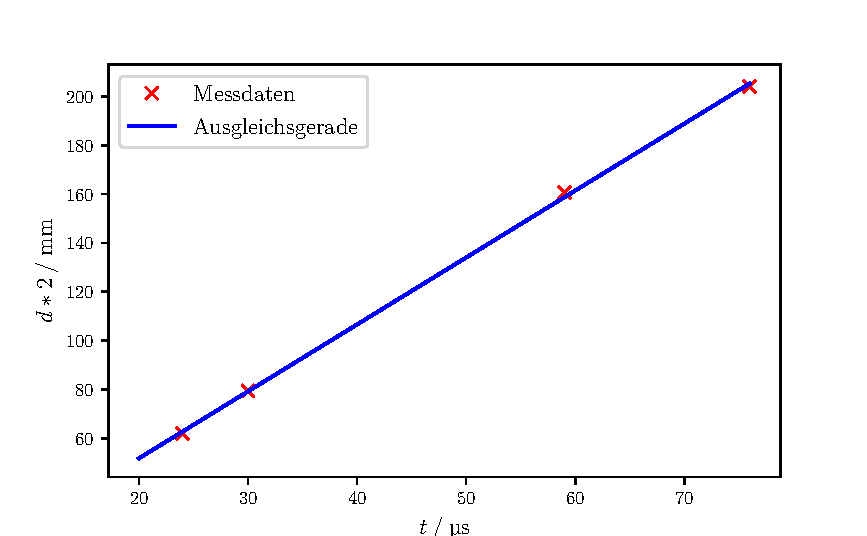
\includegraphics{build/plot1.pdf}
  \caption {Darstellung der Zylinderdicken gegen die Laufzeiten zur Berechnung der Schallgeschwindigkeiten im Impuls-Echo-Verfahren.}
  \label{fig:plot1}
\end{figure}
Die Parameter der linearen Regression und somit die bestimmte Schallgeschwindigkeit $c$ und die Dicke der Ausgleichsschicht $b$ betragen
\begin{align*}
  c_{IE}& =( 2740.76\pm 40.50 ) \si{\meter\per\second}\\
  b &= (-3.00\pm 2.10) \si{\milli\meter}.
\end{align*}


\subsection{Bestimmung der Schallgeschwindigkeit mit dem Durchschallverfahren}
\label{subsec:SchallDurchV}

Bei dieser Messreihe werden die Zylinder anhand des Durchschallungsverfahrens nach \autoref{sec:Durchführung} ausgemessen.
Die Messung wird für dieselben $4$ Zylinder wie in \autoref{sub:ImpEch} durchgeführt.
Die Messwerte der Laufzeiten und Amplituden sind in \autoref{tab:tADurch} dargestellt.

\begin{table}[H]
  \centering
  \caption{Laufzeit und Amplituden durch verschiedene Zylinder mit dem Durchschallungs-Verfahren.}
  \label{tab:tADurch}
  \sisetup{table-format=2.2}
  \begin{tabular}{S[table-format=1.0] S[table-format=2.0] S[table-format=1.2] }
  \toprule
  {Zylinder} & {Laufzeit $t / \si{\micro\second}$} &  {Amplitude $A / \si{\volt}$}\\
  1 &  13  & 1.24  \\
  2 &  15  & 1.32  \\
  3 &  30  & 1.18  \\
  4 &  38  & 0.60  \\
  \bottomrule
  \end{tabular}
\end{table}

Auch bei dieser Messung soll die Schallgeschwindigkeit $c$ berechnet werden.
Hier muss die nach $c$ umgestellte \autoref{eqn:Strecke} allerdings modifiziert werden, da der Faktor $2$ nicht mehr benötigt wird.
Dies liegt daran, dass nun nicht mehr eine Sonde als Sender und Empfänger genutzt wird und die Strecke doppelt durchlaufen wird, 
sondern an beiden Seiten des Probestücks jeweils eine Sonde anliegt und somit eine Sonde als Empfänger und die andere als Sender fungiert.
Die Berechnung erfolgt analog zu \autoref{fig:plot1} mithilfe einer Ausgleichsgerade. Diese ist in \autoref{fig:plot3} dargestellt.
\begin{figure}[H]
  \centering
  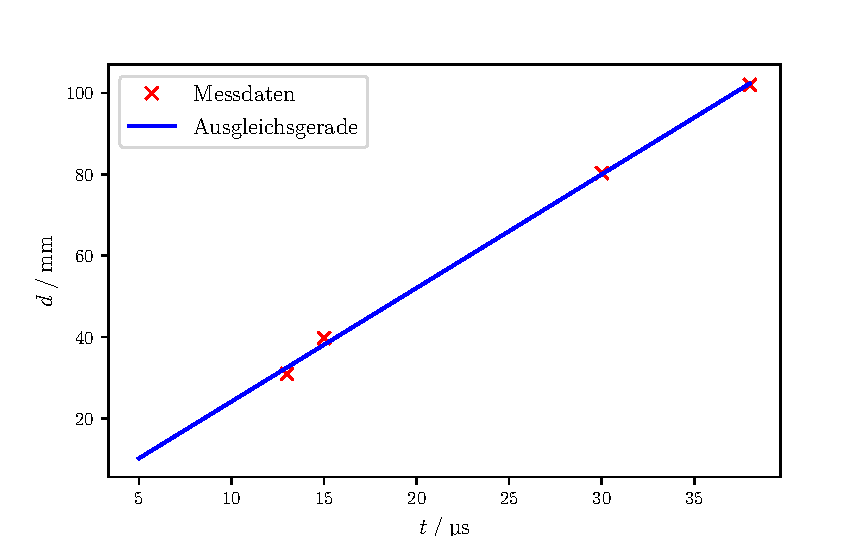
\includegraphics{build/plot3.pdf}
  \caption {Darstellung der Zylinderdicken gegen die Laufzeiten zur Berechnung der Schallgeschwindigkeiten im Durchschallungsverfahren.}
  \label{fig:plot3}
\end{figure}
Die Parameter der linearen Regression und somit die bestimmte Schallgeschwindigkeit $c$ und die Dicke der Ausgleichsschicht $b$ betragen
\begin{align*}
  c_{D}& =( 2791.47\pm 76.34 ) \si{\meter\per\second}\\
  b &= (-3.75\pm 2.00) \si{\milli\meter}.
\end{align*}

Der Ausgangsimpuls der als Sender fungierenden Sonde beträgt $A_0= \qty{1.18}{\volt}$.
Die logarithmierten Messwerte $\log{\frac{A}{A_0}}$ werden gegenüber der Zylinderdicke aufgetragen und eine 
Ausgleichsrechung der Form $\log{\frac{A}{A_0}}= -\alpha \cdot d$ durchgeführt. Die Ergebnisse sind in \autoref{fig:plot2} dargestellt.
\begin{figure}[H]
  \centering
  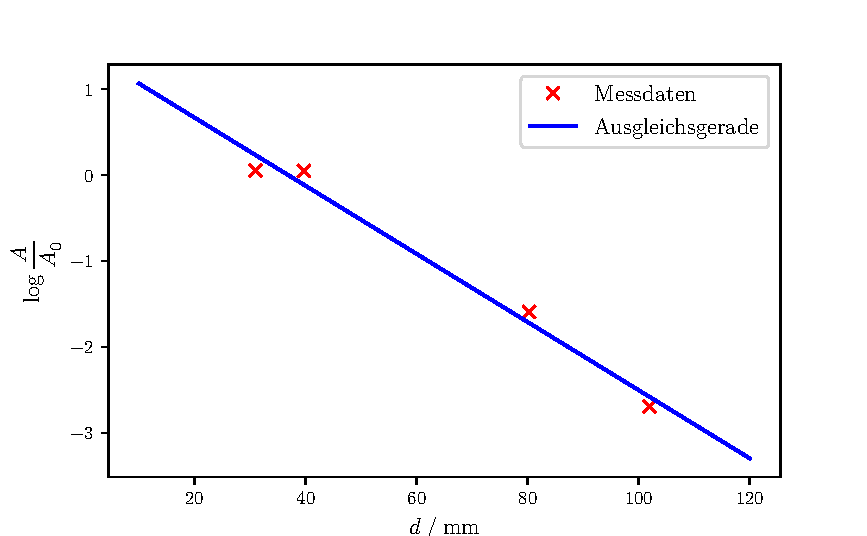
\includegraphics{build/plot2.pdf}
  \caption {Darstellung der logarithmierten Amplituden gegenüber der Zylinderdicken zur Berechnung der Dämpfung im Durchschallungsverfahren.}
  \label{fig:plot2}
\end{figure}

Der Absorptionskoeffizient ergibt sich zu
\begin{align*}
  \alpha &=( 8.99\pm 4.42) \si{\per\meter}.
\end{align*}

\subsection{Spektrale Analyse (FFT) und Cepstrum}
\label{subsec:FFT}
Nun wird die Darstellung als FFT und Cepstrum verwendet. 
Die Messung wird nach \autoref{sec:Durchführung} durchgeführt.
Aus den Laufzeiten der Peaks ergibt sich eine Dicke der Platten von 


\subsection{Biometrische Untersuchung eines Augenmodells}
\label{subsec:Augew}

\begin{figure}[H]
  \centering
  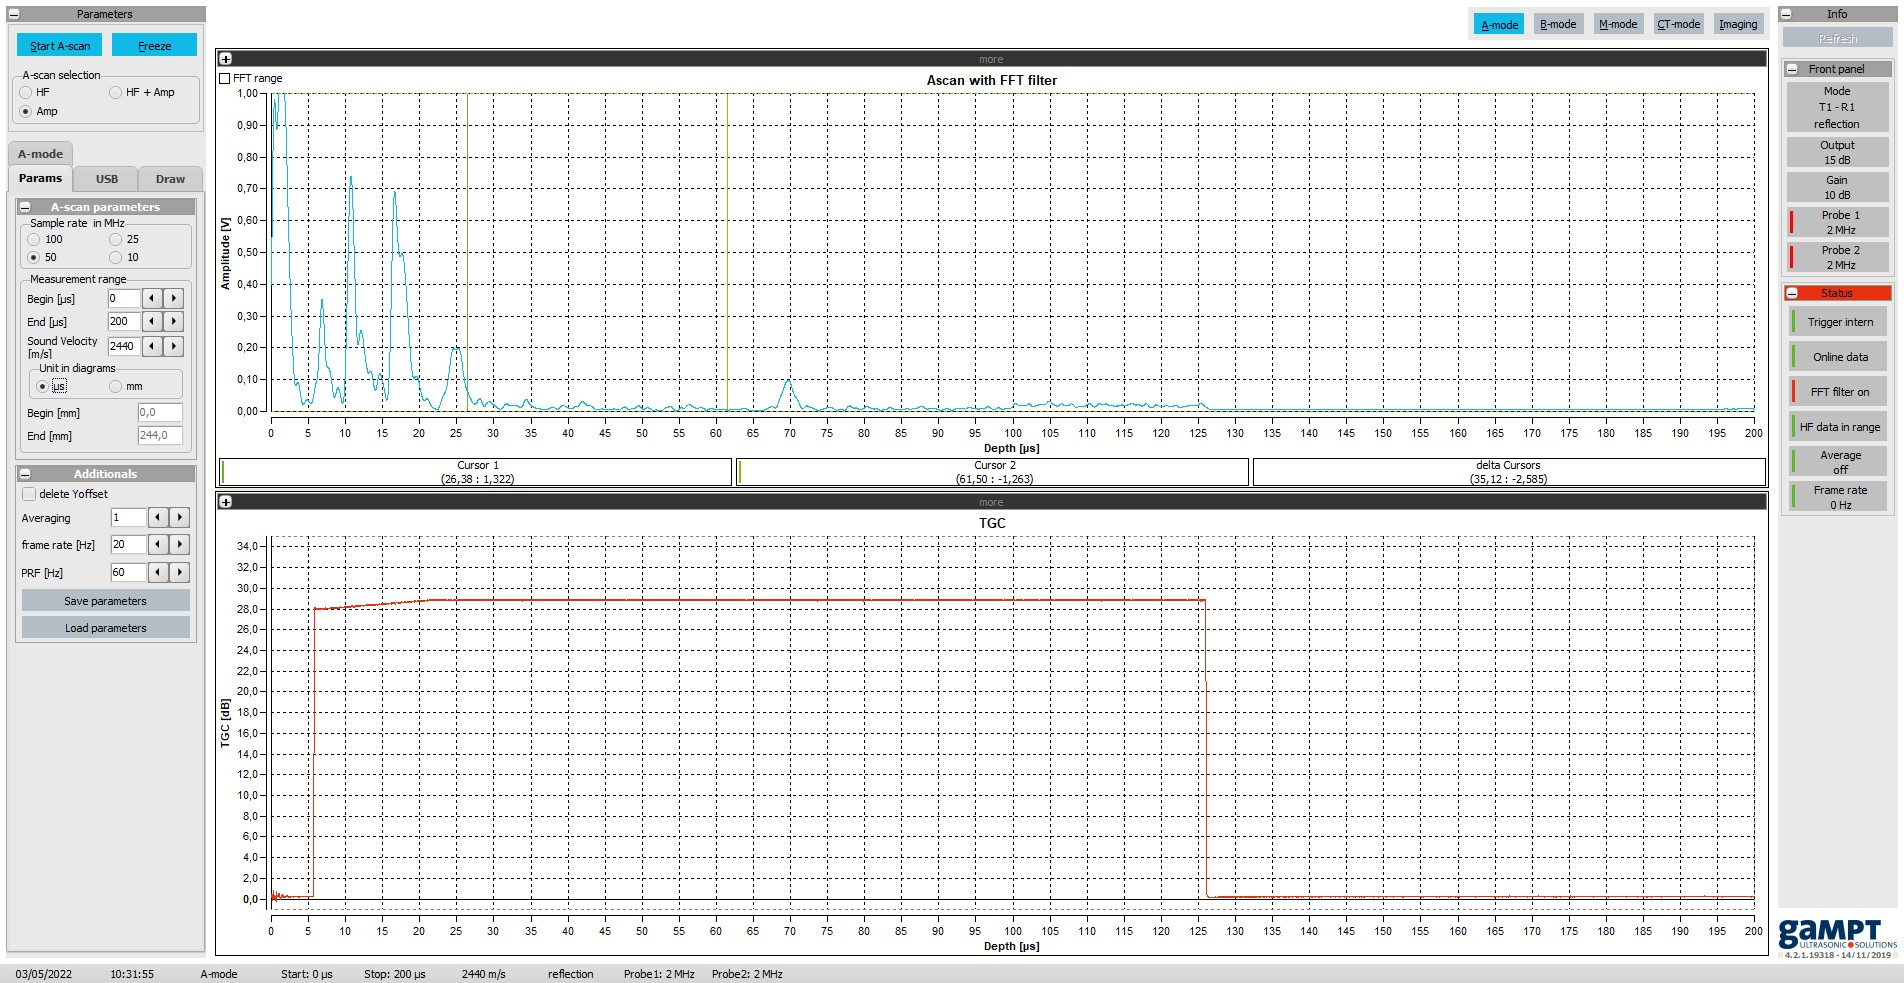
\includegraphics{build/auge.jpg}
  \caption {A-Scan des Augenmodells.}
  \label{fig:auge}
\end{figure}

Bei der Untersuchung des Augenmodells werden im A-Scan (siehe \autoref{fig:Auge}) mehrere Peaks beobachtet.
Diese lassen sich der Iris, dem Ein- und Austritt aus der Linse und der Retina zuordnen und sind in \autoref{tab:Auge} dargestellt.
\begin{table}[H]
  \centering
  \caption{Laufzeiten im Auge.}
  \label{tab:Auge}
  \sisetup{table-format=2.2}
  \begin{tabular}{c S[table-format=2.0] }
  \toprule
  {Augenbestandteil} & {Laufzeit $t / \si{\micro\second}$} \\
    Iris            &  11 \\
    Linseneintritt  &  17 \\
    Linsenaustritt  &  25 \\
    Retina          &  69 \\

  \bottomrule
  \end{tabular}
\end{table}

Mithilfe von \autoref{eqn:Strecke} werden die Maße des Augenmodells berechnet. Hierbei muss darauf geachtet werden, dass sich
die Schallgeschwindigkeit in der Linse $c_L= \qty{2500}{\meter\per\second}$ und die Schallgeschwindigkeit in der Glaskörperflüssigkeit
$c_{GK}= \qty{1410}{\meter\per\second}$ unterscheiden.

\begin{table}[H]
  \centering
  \caption{Abstände im Auge.}
  \label{tab:Auge}
  \sisetup{table-format=2.2}
  \begin{tabular}{c S[table-format=2.2] }
  \toprule
  {Augenbestandteil} & {Standort $s / \si{\milli\meter}$} \\
  Iris            &  7.76\\
  Linseneintritt  &  11.99\\
  Linsenaustritt  &  21.99\\
  Retina          &  60.77\\
  \bottomrule
  \end{tabular}
\end{table}